\documentclass[10pt,a4paper]{report}
%\special{papersize=210mm,297mm}  % for a4 make smaller the page
%\special{papersize=8.5in,11in} 	% for letter, change docClass to letter too

\usepackage[spanish,mexico]{babel} 
%\usepackage[latin1]{inputenc}
\usepackage[utf8]{inputenc}

% set double space, normal out a value = 1
%\renewcommand{\baselinestretch}{1.66}
\usepackage{setspace}

% M a r g i n s 
\usepackage[top=2.4cm, bottom=2.7cm, left=3.3cm, right=2.0cm]{geometry}   % with the script is lower the text, with kile it put +o- 1 cm above, check when pinted in the school

% controlf the page number and others
% \usepackage{fancyhdr}  % don't put this block before geometry pacage, the pag. num will be bad formatting
% \pagestyle{fancy}
% \fancyhead{}
% \fancyfoot{}
% \lhead{}
% \rhead{\today}
% \lfoot[\thepage]{}
% \rfoot[]{\thepage}
%%%%%%%%%%%%%%%%%%%%%%%%%%%%%%%%%%%%%%%

\usepackage[square, comma, sort&compress]{natbib}

\usepackage{makeidx}

% how many levels the table of contents will have 
\setcounter{secnumdepth}{3}
\setcounter{tocdepth}{3} 		

\usepackage{url}
\usepackage{subfig}  % para usar la función subfigura
\usepackage{epsfig}  % para trabajar con figs eps 

% for tables
\usepackage{multirow}
\usepackage{bigstrut}
\usepackage{booktabs}
\usepackage{rotating} 				% for vertical text in tables with  \begin{sideways}Paper\end{sideways} &\begin{sideways}Static\end{sideways} \\

\usepackage{algorithm}
%\usepackage{algorithmic}
%\usepackage{algpseudocode}

%\usepackage[colorlinks]{hyperref}  % to put links to the document in colour
\usepackage[printonlyused,withpage]{acronym}

\usepackage{hyphenat} 			%hyphenation of compound words

\usepackage{array} 			% to increse space between rows in tables using \setlength{\extrarowheight}{1.5pt}

%\usepackage{multicol}

\usepackage{pdfpages}
\usepackage{pdflscape} 			% for landscape some pages
% \begin{landscape}
% \end{landscape}

\usepackage{textcomp} 			% for the +- sign \textpm

% like verbatim but recognize commands
%\usepackage{alltt}

%textFiles/dataSets
%  \includeonly{textFiles/acroList, textFiles/intro}
% \includeonly{textFiles/acroList, textFiles/LiterReview}
% \includeonly{textFiles/acroList, textFiles/dataSets}
% \includeonly{textFiles/acroList, textFiles/epnetAlg, textFiles/AppA}
% \includeonly{textFiles/acroList, textFiles/evoMNN}%, textFiles/AppB}
% \includeonly{textFiles/acroList, textFiles/moduleReuse, textFiles/conc}

%\includeonly{textFiles/acroList, textFiles/intro, textFiles/LiterReview, textFiles/moduleReuse}

%\includeonly{textFiles/acroList, textFiles/conc}

\graphicspath{ {images/} }


\makeindex

\begin{document}
    
    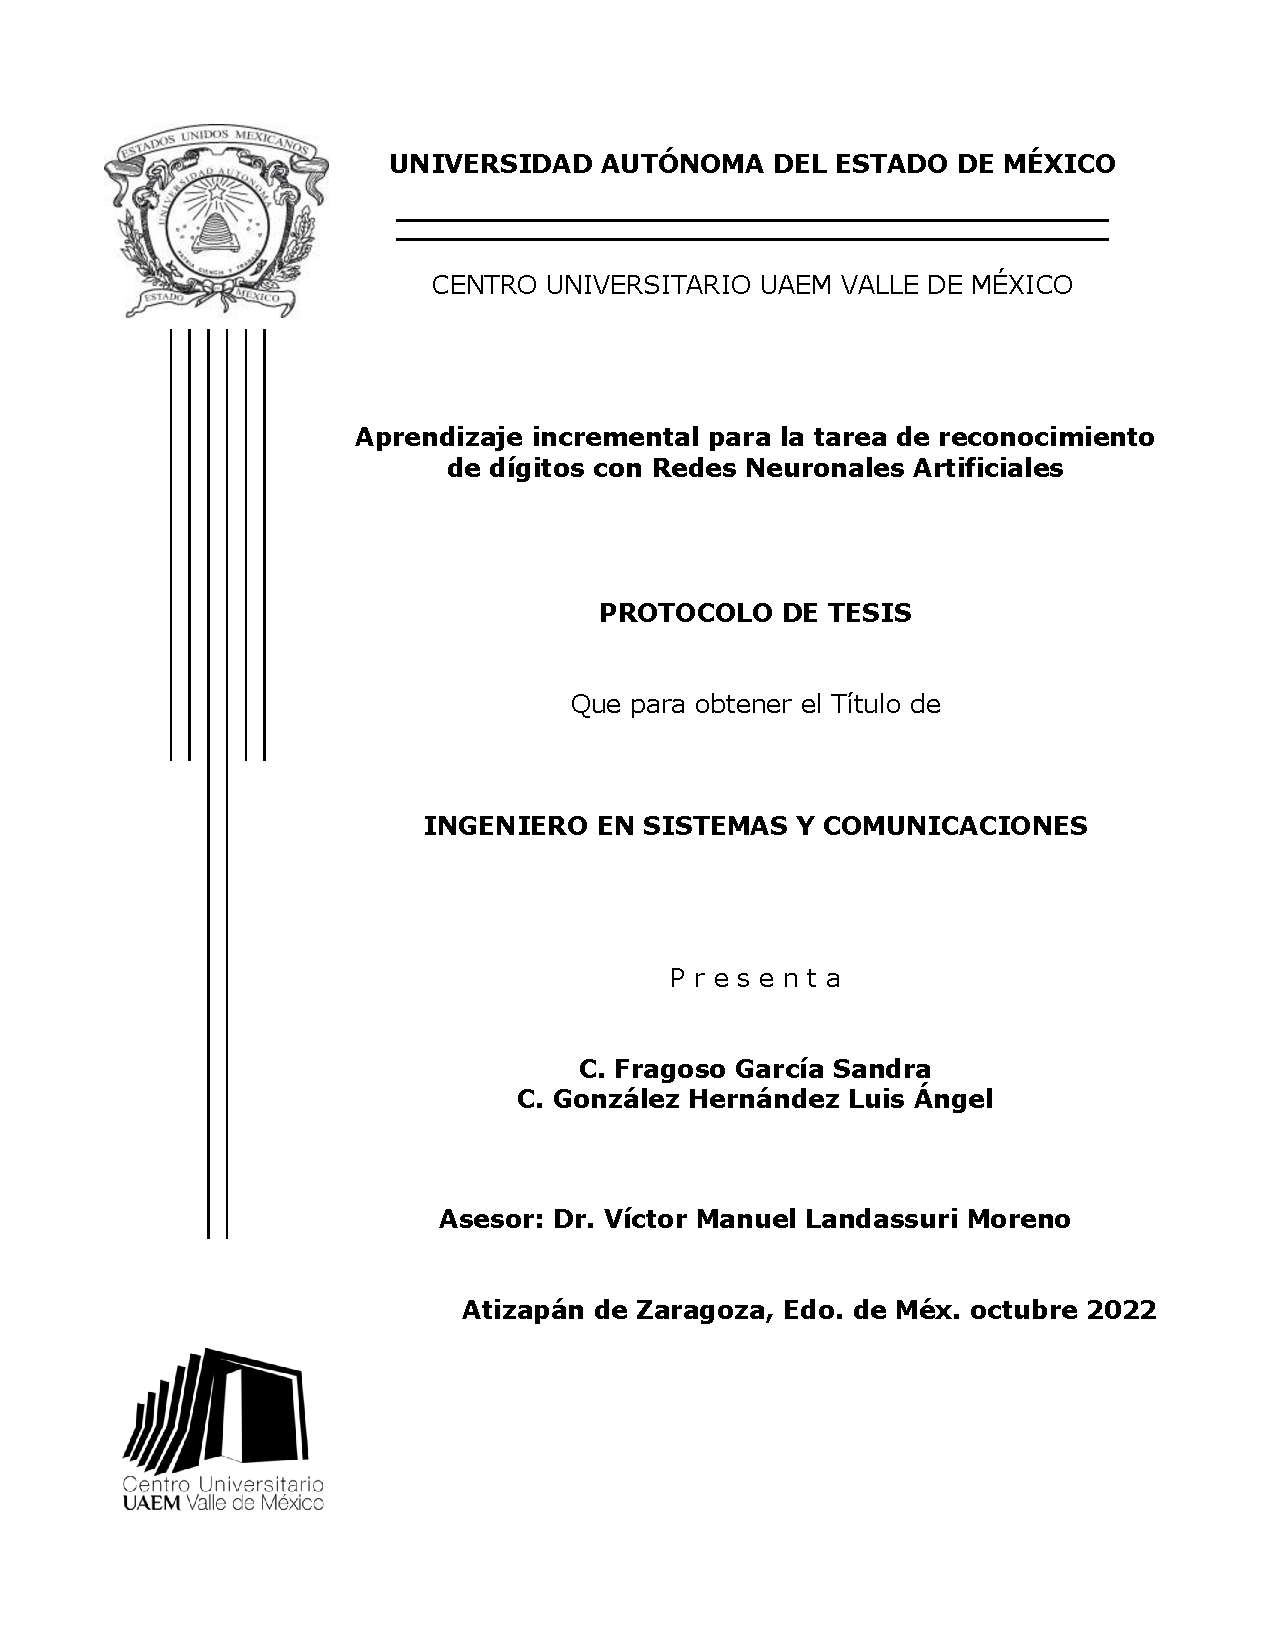
\includepdf{textFiles/portada.pdf}
    \tableofcontents

    \listoffigures
    
    \section{Introduccion}

El aprendizaje incremental es un método el cual a sido implementado en el área de la inteligencia artificial, ya que al realizar tareas especificas de dicha rama nos 
ayuda a optimizarla para que el algoritmo sea más eficiente.
Cualquier tipo de aprendizaje puede ser considerado aprendizaje incremental si el problema a resolver tiene un entrenamiento simple, adem\'as este tipo de algoritmo es conocido como \textit{algoritmo lineal sin memoria},
en la mayor\'ia de los casos este tipo de aprendizaje es el preferido o favorito por los desarrolladores \cite{GiraudCarrier2000}.

Las redes neuronales artificiales (RNAs) son procesos matem\'aticos los cuales son utilizados en el \'area de Machine Learning para 
la resoluci\'on de problemas no lineales, estos deben de pasar por una funci\'on de activaci\'on la cual es una multiplicaci\'on 
entre lo valores otrogados, al ser procesados por las capas que contenga la neurona, obtendremos un valor distinto al de entrada.

Adem\'as son una distribuci\'on muy conocida de parte del Machine Learning, de otra manera es el poder que tienen las computadoras para una buena estructura distribuida en paralelo y una buena habilidad de aprendizaje, 
este modelo computacional se define por medio de las neuronas biologicas las que son encargadas de que el ser humano pueda aprender o distinguir de distintos aspectos, este tipo de 
metodo es motivado para poder obtener la meta de un buen aprendizaje de maquina \cite{liu2015}.

Un factor importante para esta rama es la perdida de memoria, este es un problema biol\'ogico, el cual tanto afecta a los humanos como a las maquinas, es por eso que se han elaborado distintos
experimentos para poder convatir esta problematica.
Uno de  estos es el caso de John Bullinaria, quien maneja la arquitectura de doble peso, ya que en su experimento da a notar que mejora la utilizaci\'on del aprendizaje incremental, esto se logro 
con sistemas existentes como lo es Learn++.

Cabe mencionar que el experimento realizado fue un problema de generalizaci\'on m\'as comunes, pero se necesitan m\'as evidencias 
de que usando esta metodolog\'ia sirve para utilizarlo no solamente en tareas generalizadas, adem\'as se espera un mejor rendimiento \cite{Bullinaria2009}.  \\


\section{Planeamiento}

    Indicar de forma general como es el funcionamiento de las redes neuronales en el uso general, como es que se produce la falta de memoria en 
    estos modelos de predicciones. Poner en pr\'actica los modelos de experimentación de John Bullinaria para comprobarlos con
    problematicas m\'as robustas y optimizarlo para que sea un m\'etodo eficiente.
    \section{Planeamiento}

    Las Redes Neuronales Artificiales tienen la habilidad de poderse aprender una tarea, 
    y poder hacer o resolver tareas de predicción o clasificación básicamente. En este 
    sentido, con algoritmos de aprendizaje como el Backpropagation, permite ajustar los 
    pesos de una RNA para que esta pueda empezar a resolver una tarea particular.  No 
    obstante, muchas de las tareas que se resuelven en la vida diaria, van generando mas 
    información con el tiempo, por ejemplo, el comportamiento de un una serie financiera, 
    o bien la predicción del clima en una determinada región. Así,  se tiene el aprendizaje 
    incremental, siendo un método poco explorado,  enfocado en poder aprender nueva información del 
    problema, sin tener que volver a entrenar todo el modelo con la información anterior, y la 
    nueva que acaba de llegar, esto es, en los modelos actuales de aprendizaje máquina, si se usa 
    un conjunto de datos para entrenar un modelo en especifico, dicho modelo es funcional para 
    dicho conjunto de datos y la información que ello representa. Sin embargo, si es necesario 
    incorporar nueva información al modelo, es necesario recolectar dicha información nueva, 
    agregarla a la que se tenia anteriormente, y volver a entrenar todo el modelo para que \'este 
    pueda incorporar la nueva información.

    De esta forma, una red ya entrenada con un primer conjunto de datos $d_{1}$ se desea entrenar 
    con un nuevo conjunto de datos del mismo problema $d_{2}$, al entrenar la red con $d_{2}$ se 
    perderá en conocimiento aprendido por $d_{1}$.  Si no se desea utilizar un modelo de aprendizaje 
    incremental, se tendría que juntar el conjunto $d_{1}$ y $d_{2}$ en un solo conjunto y volver a 
    entrenar la RAN para así poder incorporar el nuevo conocimiento ($d_{2}$) a la RNA. Si se desea 
    utilizar el método de aprendizaje incremental, se puede entrenar en un primer moemnto a la red 
    con el conjunto $d_{1}$, posteriormente con $d_{2}$ teniendo poca perdida de información de $d_{1}$. 
    Si más adelante llega mas información del problema ($d_{3}$) que se desee incorporar a la base 
    de conocimientos de la RNA, entonces solo habrá que entrenar la RNA con $d_{3}$ usando el modelo 
    incremental para tener una p\'erdida mínima de información de $d_{1}$ y $d_{2}$. 

    De esta forma, el presente trabajo tomar\'a como base la investigación de \cite{bullinaria2009}, 
    en donde utiliza una configuración de pesos dobles (a una RNA se duplican todos sus pesos), 
    donde a una capa de pesos duplicados se enlaza con una tasa de aprendizaje alta, para simular un 
    rápido aprendizaje, y por ende simular lo que sería memoria a corto plazo. En su contraparte, 
    la segunda capa de pesos duplicados, se enlaza con una tasa de aprendizaje baja para aprender 
    lentamente un problema, simulando la memoria a largo plazo.  Es decir, al momento de aprender una 
    tarea nueva,  una capa de pesos aprenderá muy rápido la nueva tarea (tasa alta de aprendizaje) y 
    por ende olvidará más rápidamente los datos ya aprendidos anteriormente, por otro lado, la segunda 
    capa de pesos duplicados, aprenderá muy lentamente los nuevos datos que llegan, y por ende olvidando 
    poco la información que anteriormente se aprendió.  Considerando ello y también que la 
    RNA trabaja en conjunto con ambas capas de pesos duplicados, se pondera la salida de la RNA para 
    que pueda contemplar la información nueva que se acaba de agregar a la RNA, en ambas capas, así como 
    la información que se acaba de olvidar de ambas capas de pesos.

    El problema principal del aprendizaje incremental mostrado en \cite{bullinaria2009}, es que entre 
    más conjuntos de datos nuevos que lleguen, mas se olvidaran los primeros conjuntos que se aprendieron, 
    lo cual no es tan útil si se contempla que en el futuro de una RNA podrán existir 10 o 20 etapas de 
    entrenamiento incremental con nuevos conjuntos de datos que se vayan recolectando.

    Por ello es indispensable poder explorar nuevas configuraciones de RNAs que permitan mejorar los 
    métodos actuales para permitir una menor cantidad de olvido conforme llegue nueva información al 
    modelo. Donde al igual que en trabajos anteriores,  el presente trabajo se basará en conceptos de 
    memoria a corto y largo plazo, y en lugar de hacer una copia de los pesos actuales y tener dos 
    tasas de aprendizaje, una rápida para simular la memoria a corto plazo, y otra tasa de aprendizaje 
    para simular la memoria a largo plazo, se explorará por hacer mas copias de los pesos, teniendo más 
    tasas de aprendizaje que operen en cada una de dichas copias.
    
    \section{Marco Teórico}

    
    
    \subsection{Redes Neuronales Artificiales}
        
        Las redes neuronales artificiales (RNA) son procesos los cuales contienen simples unidades de procesamientos. \\
        Como podemos darnos cuenta, al mencionar RNA lo primero que se nos viene a la mente es el procesamiento biol\'ogico por el que transita el 
        cerebro humano. El m\'etodo principal de las redes neuronales es sacarle el máximo poder a los algoritmos de aprendizaje maquina, ya que las redes neuronales 
        tiene un antecedente biol\'ogico.

        Tiene demasiadas (EN LUGAR DETIENEN, PUEDEN DECIR: LAS RNAS PRESENTAN) utilidades las cuales ayudan a distintas (ELIMINEN LA PALABRA DISTINTAS, POSIBLEMENTE TAMBIÉN ELIMINA LA PALABRA ALGUNAS, SON PALABRAS MUY GENÉRICAS QUE PRÁCTICAMENTE NO DICE NADA,MEJOR DIGAN: PUEDEN RESOLVER PROBLEMAS COMO LOS SIGUIENTES) problemáticas, algunas de las funciones que tiene son \cite{liu2015}:

(CONSIDERANDO UNO DE LOS COMENTARIOS QUE LES HAGO MÁS ARRIBA, ELIMINEN ESTOS LISTADOS Y DEJEN TODO ESCRITO EN LA FORMA DE PÁRRAFOS)
        \begin{enumerate}
            \item No linealidad.
            \item Mapeo entrada-salida.
            \item Aprendizaje robusto a errores en los datos de entrenamiento. 
            \item Entre otros.
        \end{enumerate}

        Existen varios tipos de Redes Neuronales tales como: 
        \begin{itemize}
            \item Redes Neuronales de Perceptr\'on Multicapa.
            \item Redes Neuronales Convolucionales.
            \item Entre otras.
        \end{itemize}
    
        \subsection{Redes Neuronales de Perceptr\'on Multicapa}

(REVISAR REDACCIÓN Y MEJORARLA)
            Al momento de mapear el progreso de una red nos sirve para conocer buscar un camino adecuado entre la capa de entrada y salida, esto se puede hacer 
            con problemas de una sola neurona, pero no se pueden resolver problemas no lineales, es aqu\'i donde entran los perceptrones
            multicapas, los cuales rompen con esta limitaci\'on.

            Estas neuronas est\'an compuestas de 3 capas como se puede ver en la Figura \ref{fig:fig1}:
            \begin{enumerate}
                \item Capas de entrada.
                \item Capas ocultas.
                \item Capas de salida.
            \end{enumerate}

            Los datos de entrada se van a ir propagando capa por capa, hasta llegar a la capa final, donde la información pasará
            por una funci\'on de activaci\'on la cual poermite tener en un rango controlado los valores que se propagan por la red. Al final, las neuronas de la capa de salida darán el resultado esperado o muy proximo a él, si el valor no es correcto, se deberá proceder a una etapa de entrenamiento \cite{liu2015}.

            \begin{figure}[H]
                \centering
                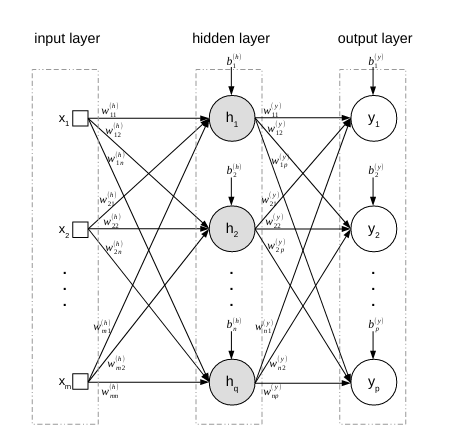
\includegraphics[width=\columnwidth]{MLP.png}
                \caption{Red Neuronal de Perceptr\'on Multicapa \cite{liu2015}}
                \label{fig:fig1}
            \end{figure}

\subsection Algoritmo Backpropagation
(Aquí describan este algoritmo, la página que les pase de John les puede ayudar. Términos importantes de escribirlo porque sobre él se basaron para hacer la implementación de las redes con pesos duplicados)


        \subsection{Redes Neuronales Convolucionales}

            Este tipo de red trabaja con el uso de imágenes, por lo general de alta calidad, el \'unico problema que se tiene 
            al momento de que sean de alta resoluciones son:
            \begin{itemize}
                \item El tiempo de entrenamiento sea enorme.
                \item El tiempo de testo sea muy tardío.
            \end{itemize}

            Consta de diversas multicapas alternadas, al final tiene una red perceptr\'on multicapa. (Revisen la redacción, está muy segmentada las ideas, tienen que explicar un poco más para que se entienda mejor, tomen como base la redacción que les pongo al inicio del trabajo, vean cómo voy a explicando más cosas, y aunque me llevo más espacio, queda mejor)
            La entrada de una red convolucional, con diferentes medidas en altura y anchura de imagen, para el uso 
            de los proyectos se trabajan en escalas de grises, las cuales contienen filtros y cada filtro tiene distintos 
            rasgos y características de tamaño. Cada capa es submuestreo de m\'inimo a m\'aximo, muestra donde se toman valores 
            desde 2 im\'agenes pequeñas hasta no mas de 5 im\'agenes grandes.

            Antes o despu\'es del submuestreo se aplica la activaci\'on sigmoidal para cada mapeo de rasgos \cite{duran2017}.

            \begin{figure}[H]
                \centering
                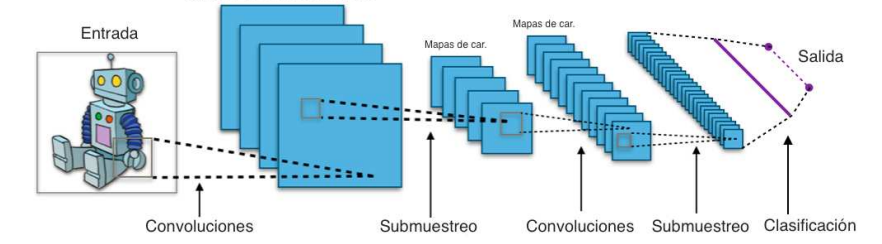
\includegraphics[width=\columnwidth]{esquemaRedConvolucional.png}
                \caption{Esquema de una Red Convolucional \cite{duran2017}}
                \label{fig:fig2}
            \end{figure}

Así como las redes convolucionales, también existen las redes profundas(deep learning), sin embargo, como se comenta en esta sección \label{sec:delimitation} el presente trabajo solo se basará en redes del tipo multicapa perceptron usando el algoritmo de bacpkpropagation, donde de ser demostrado los principios aquí descritos,  se podrá aplicar a cualquier otro tipo de algoritmo de aprendizaje.  (LUIS Y SANDRA, AGREGUEN A LA DELIMITACIÓN LO QUE ESTOY INDICANDO AQUÍ, PARA QUE TENGA SENTIDO ESTO)



\section{Aprendizaje}

\subsection {Aprendizaje en humanos}
        El humano tiene una forma de aprendizaje muy particular, la cual se basa del estudio, donde lee, escribe y practica acerca de
        su tema de interés, pero dicho aprendizaje se puede ir olvidando, esto es una acción muy común que a cualquier persona le sucede.
        Existen estudios donde se comenta que existen tres motivos del porque se olvidan las cosas, proviene parte de la regularización de las emociones,
        el como se adquirieron los conocimientos, y porque el olvido es un proceso por el cual el ser humano transita a lo largo de su vida \cite{Nrby2015}. Pero cabe
        mencionar que esto no es lo único que causa la perdida de memoria, ya que existe la déficit de memoria. 

    \subsection{Aprendizaje Humano}
        Al momento de hablar del aprendizaje humano, se debe de hablar de la ciencia cognitiva, que es quien se encarga de descubrir esta incógnita,
        esta ciencia lo estudia de un modo multidisciplinario, el cual abarca las \'areas de \cite{bransford2000}: 
        \begin{itemize}
            \item La antropología.
            \item La lingüística.
            \item La filosofía.
            \item La sicología del desarrollo.
            \item La ciencia de la computación. 
            \item La neurociencia.
        \end{itemize}
        Con el método de esta ciencia se pueden descubrir dos tipos de aprendizaje que son:
        \begin{enumerate}
            \item Aprendizaje con Compresi\'on.
            \item Aprendizaje Activo.
        \end{enumerate}
        \subsubsection{Aprendizaje con Compresi\'on}
            La comprensi\'on es una actividad la cual se ha generado al momento de realizar cualquier tipo de lectura.\\
            Al hablar de este tema nos enfocamos en el \'ambito estudiantil que es donde m\'as se maneja esta t\'actica, esto es una
            practica algo compleja, sistemática y organizada, ya que nos da el significado de la literatura, gracias a esto se puede
            obtener el contexto de la literatura.

            Al conocer esto podemos decir con seguridad que para cualquier tipo de aprendizaje la comprensi\'on es 
            una parte primordial \cite{perez2014}.

        \subsubsection{Aprendizaje Activo}
            El aprendizaje de la forma en la que se conoce no es del todo efectiva, ya que el sistema educativo
            no se basa en el principio de \textit{belongingness}, el cual esta asociado al estimulo con su respuesta,
            y esto es lo m\'as importante para que el ser humano pueda aprender cualquier cosa.\\
            Este tipo de aprendizaje se basa en la recepci\'on de conocimientos y la pr\'actica donde se ponen en marcha los conocimientos adquiridos.\\
            Otro concepto importante aqu\'i es la tautolog\'ia doble (\textit{selbstt\"atiges Lernen}), que en palabras informales es convertirse en autodidacta, 
            se puede observar que esto pertenece a dicho aprendizaje, porque usa el principio mencionado anteriormente \cite{Huber2008}.
   

 \subsection{Aprendizaje Incremental}
        Con el pasar de los años la tecnología a evolucionado, eso quiere decir que el Aprendizaje Automático se ha actualizado, que la 
        cantidad de datos va aumentado con más frecuencia.
        
        Se puede verificar como \textit{"Una tarea de aprendizaje es incremental si los ejemplos de entrenamiento usados para 
        resolverla están disponibles en horas extras, generalmente uno a la vez"} \cite{GiraudCarrier2000}, si los resultados no se 
        necesitan de manera urgente, este tipo de trabajos serán resueltos por algoritmos de aprendizaje no incremental. 

        Una área donde esto es de mucha utilidad es la \textit{Rob\'otica} porque este necesita estar en constante entrenamiento \cite{GiraudCarrier2000}.

        Dicha forma de aprender fue inspirada en la forma que el humano aprende y esta es una forma más rápida, fue por esto que fue adoptada 
        por el aprendizaje maquina.

        Con el paso del tiempo se ha convertido en un paradigma del aprendizaje automático, aquí el aprendizaje toma el lugar de nuevos ejemplos para juntarlos 
        y conforme van aprendiendo estos toman el lugar de los ejemplos ya aprendidos \cite{liu2015}.

        \subsubsection{Algoritmos de Aprendizaje Incremental}
            \textit{"Un algoritmo de aprendizaje es incremental si,
            para cualquier muestra de entrenamiento dada:
            \begin{equation}
                e_{1} , .... , e_{s}
			\end{equation}
            , produce un secuencia de hipótesis 
            \begin{equation}
                h_{0} , h_{1}, . . . , h_{n} 
            \end{equation}
            , tal que hi+1 depende solo de hola y del ejemplo actual e"} \cite{GiraudCarrier2000}, como se 
            observa, estos son algoritmos que permiten a la inteligencia artificial poder realizar actividades de predicci\'on 
            de una manera m\'as eficaz.\\
            Un ejemplo del uso de esta rama es el proyecto \textit{COBWEB}, donde se trata de categorizar el n\'umero de Cl\'uster y la pertenencia 
            de dichas categor\'ias por medio de una m\'etrica probabil\'istica global, esto lo realiza por medio de que se agrega 
            una nueva categor\'ia, este proceso lo que realizar\'a es actualizar todas las probabilisticas con los nuevos datos recabados \cite{fisher1987}.

Aquí falta describir a detalle cómo se lleva acabo el aprendizaje incremental, se pueden basar en el trabajo de Bullinaria y Leanr ++, expliquenlo a detalle para que sea su estado del arte

    \section{Hipótesis}
    Al tener m\'as de dos capas de pesos duplicados con sus respectivas tasas de aprendizaje, permite tener un menor olvido de la información previa aprendida, en un modelo de aprendizaje incremental con redes neuronales artificiales del tipo MLP, al usar el algoritmo de Backpropagation.  
%(AQUÍ DE FAVOR SÓLO REVISA QUE EL ACRÓNIMO MLP - MULTI CAPA PERCEPTRON DEL INGLES MULTILAYER PERCEPTRON - SE HAYA DESCRITO ANTERIORMENTE)
    \section{Metodología}
    El primer paso a realizar en esta investigación es recrear el código mostrado en \cite{bullinaria2009}, donde se describe la implementación de una red  neuronal multicapa usando el algoritmo de entrenamiento backpropagation en el lenguaje de programación Python.  Para esto se utilizará el conjunto de datos de Optical Digits,  en donde se tendrá que preprocesar los datos, para eliminar registros inválidos. 

    Posteriormente se implementará una nueva versión del código en donde se experimentará con mas de dos capas de pesos duplicados para mejorar la tasa de olvido de información al momento de usar el aprendizaje incremental.  Para ello se explorará incrementando gradualmente el nueron de capas (esto no lo entendi,neuronas de capas?)de pesos duplicados, hasta llegar al punto en que mas capas no generen un decremento de las tasas de olvido/error.

(REVISEN LA REDACCIÓN Y MEJORENLA DE FAVOR)
    Cuando los dos proyectos se tengan, se realizar\'a una comparación, donde se ver\'a cual de estos dos experimentos
    es más eficaz en proyectos de la vida real.
    
\section{Cronograma de Actividades}
(EL CRONOGRAMA DE ACTIVIDADES DICE JOHN BULLINARIA EN LA PARTE DE ARRIBA, ELIMINAR ESO)

    \begin{figure}[H]
        \centering
        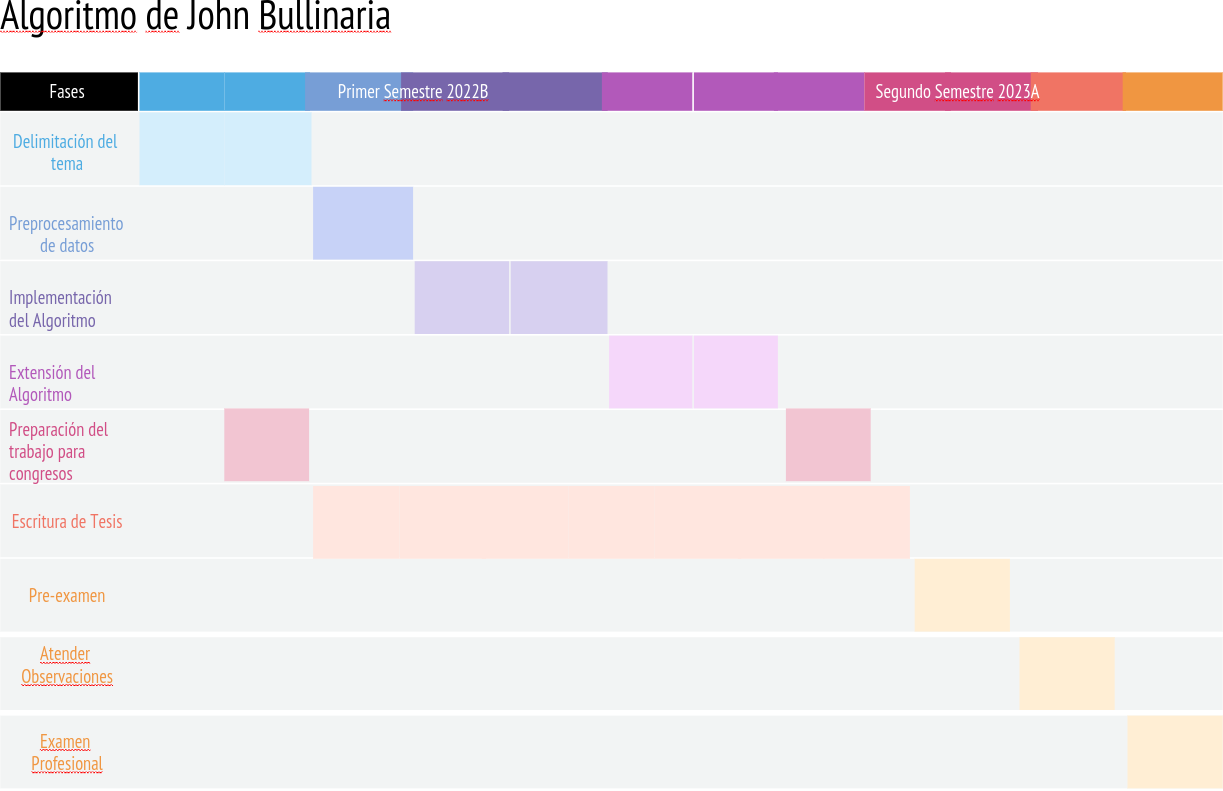
\includegraphics[width=\columnwidth]{diagramaGantt.png}
        %\caption{Elimine estoa horita, no hace falta ponerle un titulo, dado que es la únic figura en la sección}
        \label{fig:fig3}
    \end{figure}

\section{Organización del Capitulado}


	En el capitulo 2 se ver\'a lo que es el aprendizaje humano y el aprendizaje incremental con sus algoritmos, se describirán las redes neuronales artificiales.

En el capitulo 3 se implementar\'a el articulo de John A. Bullinaria, como funciona, resultado que da al pasar los datos que dice para comprobar que funciona como menciona en su art\'iculo. En el capitulo 4 se explicar\'a como se hará la modificación a su algoritmo, cuantas capas se van a poner, como se van a repartir las tazas de aprendizaje.

Posteriormente en el capitulo 5 se mostrar\'a una comparación de los resultados de ambos trabajos. En el capitulo 6 se verán las conclusiones y trabajo futuro.

    
    %\printbibliography  
    %\bibliographystyle{acm}
    \bibliographystyle{ieeetr}%plain}
    \bibliography{bibliography}
    %\bibliography{BaseDatos2}
\end{document}
